%!TEX root = ../document.tex

\section[User Testing and Feedback (Author: Thomas B\"unger)]{User Testing and Feedback}
\label{sec:USER_TESTING}

We were able to test our paper prototype with the students from both Bachelor's project teams of the HPI EPIC chair(Figure \ref{fig:user_testing}). Both teams develop applications based on SAP's HANA technology and also faced problems similar to the ones we had discovered during our interviews. One team investigates \emph{In-Memory Data Management for Enhanced ERP} while the other focuses on \emph{Real-time Analysis of Genome Data}.

\begin{figure}
\begin{centering}
    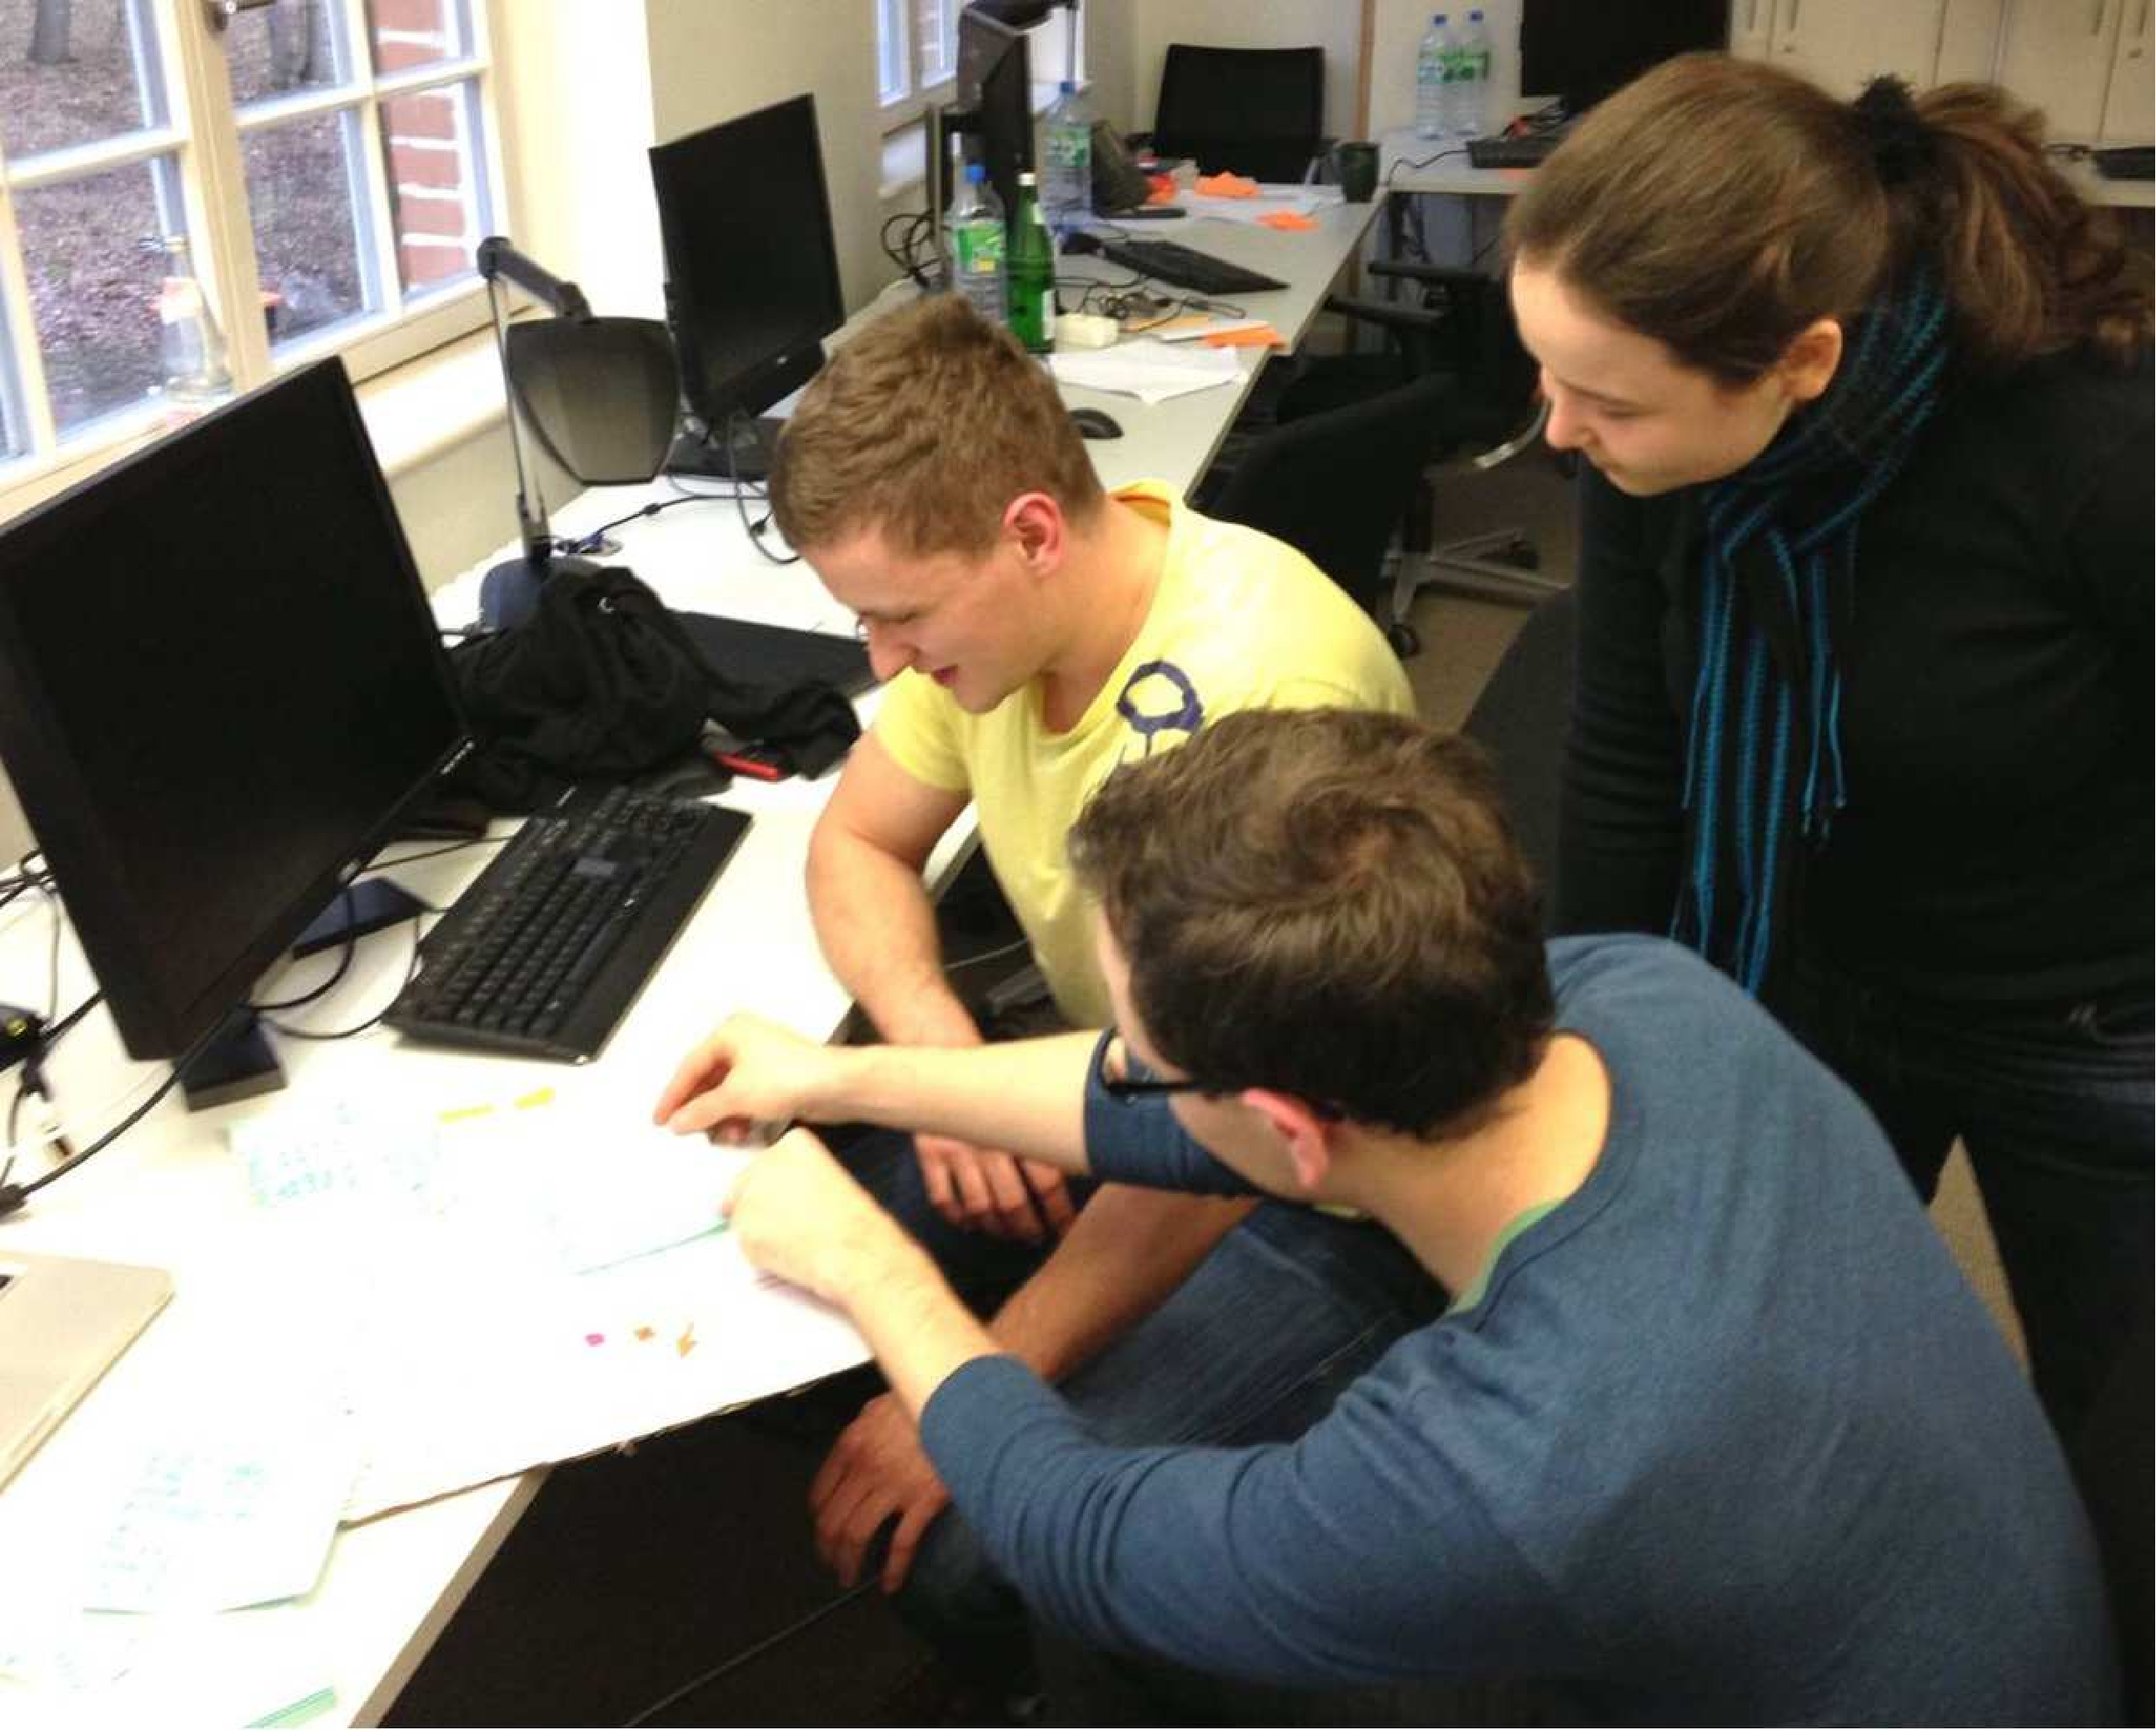
\includegraphics[width=1.0\linewidth]{images/user_testing}
    \caption{User testing with the Bachelor's project team HP2.}
    % #selfrespect
    \label{fig:user_testing}
\end{centering}
\end{figure}

In the following we present their feedback as well as general insights we gained during the 5-day-workshop that was part of the seminar as well as from Hasso Plattner and some of the tutors.

\subsection{Feedback from Bachelor's Project HP1}
\label{subsec:FeedbackBPHP1}
\begin{itemize}
	\item The team generally welcomed the idea of popup windows, but criticized the fact that they occlude parts of the underlying code. Even if detachable ones that could be freely positioned on the screen would still lead to a cluttered workspace and thus result in an inferior workspace.

	\item For maximum productivity they rather prefer keyboard shortcuts instead of the mouse pointer to interact with the data entities in the code.

	\item Developers appreciate tidy screens, even on nowadays large monitors. Hence, the amount of provided information is to be treated with care.
\end{itemize}

\subsection{Feedback from Bachelor's Project HP2}
\label{subsec:FeedbackBPHP2}
\begin{itemize}
	\item The students find the concept of a Data Context hard to grasp when presented initially.

	\item They liked the immediate feedback in the Data Context Panel as well as the warning or hint symbols that appear next to a context, when some of their code changes resulted in unintended behavior on other contexts.

	\item They wished the Data Context Panel would also include all relevant test cases, so any additional testing tools to run their test suite would become expendable.
\end{itemize}


\subsection{General Feedback during the 5-day-worshop}
\label{subsec:FeedbackWeek}
\begin{itemize}
	\item The code as well as the provided data have to be as tangible as possible and the whole editor as easily navigable as todays mobile and tablet apps.

	\item Once the number of Data Contexts increases, some clever selection mechanism or at least a searching interface might become indispensable.

	\item In addition to whole tables, the inspection of partial queries would be desirable as well.
\end{itemize}

\subsection{Feedback evaluation}
\label{subsec:FeedbackEvaluation}
As shown in Figure \ref{fig:user_feedback}, we categorized the feedback into positive and negative, identified open questions as well as some new ideas worth to explore. Some of the ideas described in Chapter \ref{sec:IDEATION} originate from this feedback evaluation step.

For the next iteration of our prototype, we removed the table inspection popup windows and instead reserved a fixed panel at the bottom to display their content. Besides the user interface we added a new field of attention: investigating different mechanisms for handling large numbers of Data Contexts - regarding the acquiring as well as the relevance filtering and selection.

\begin{figure}
\begin{centering}
    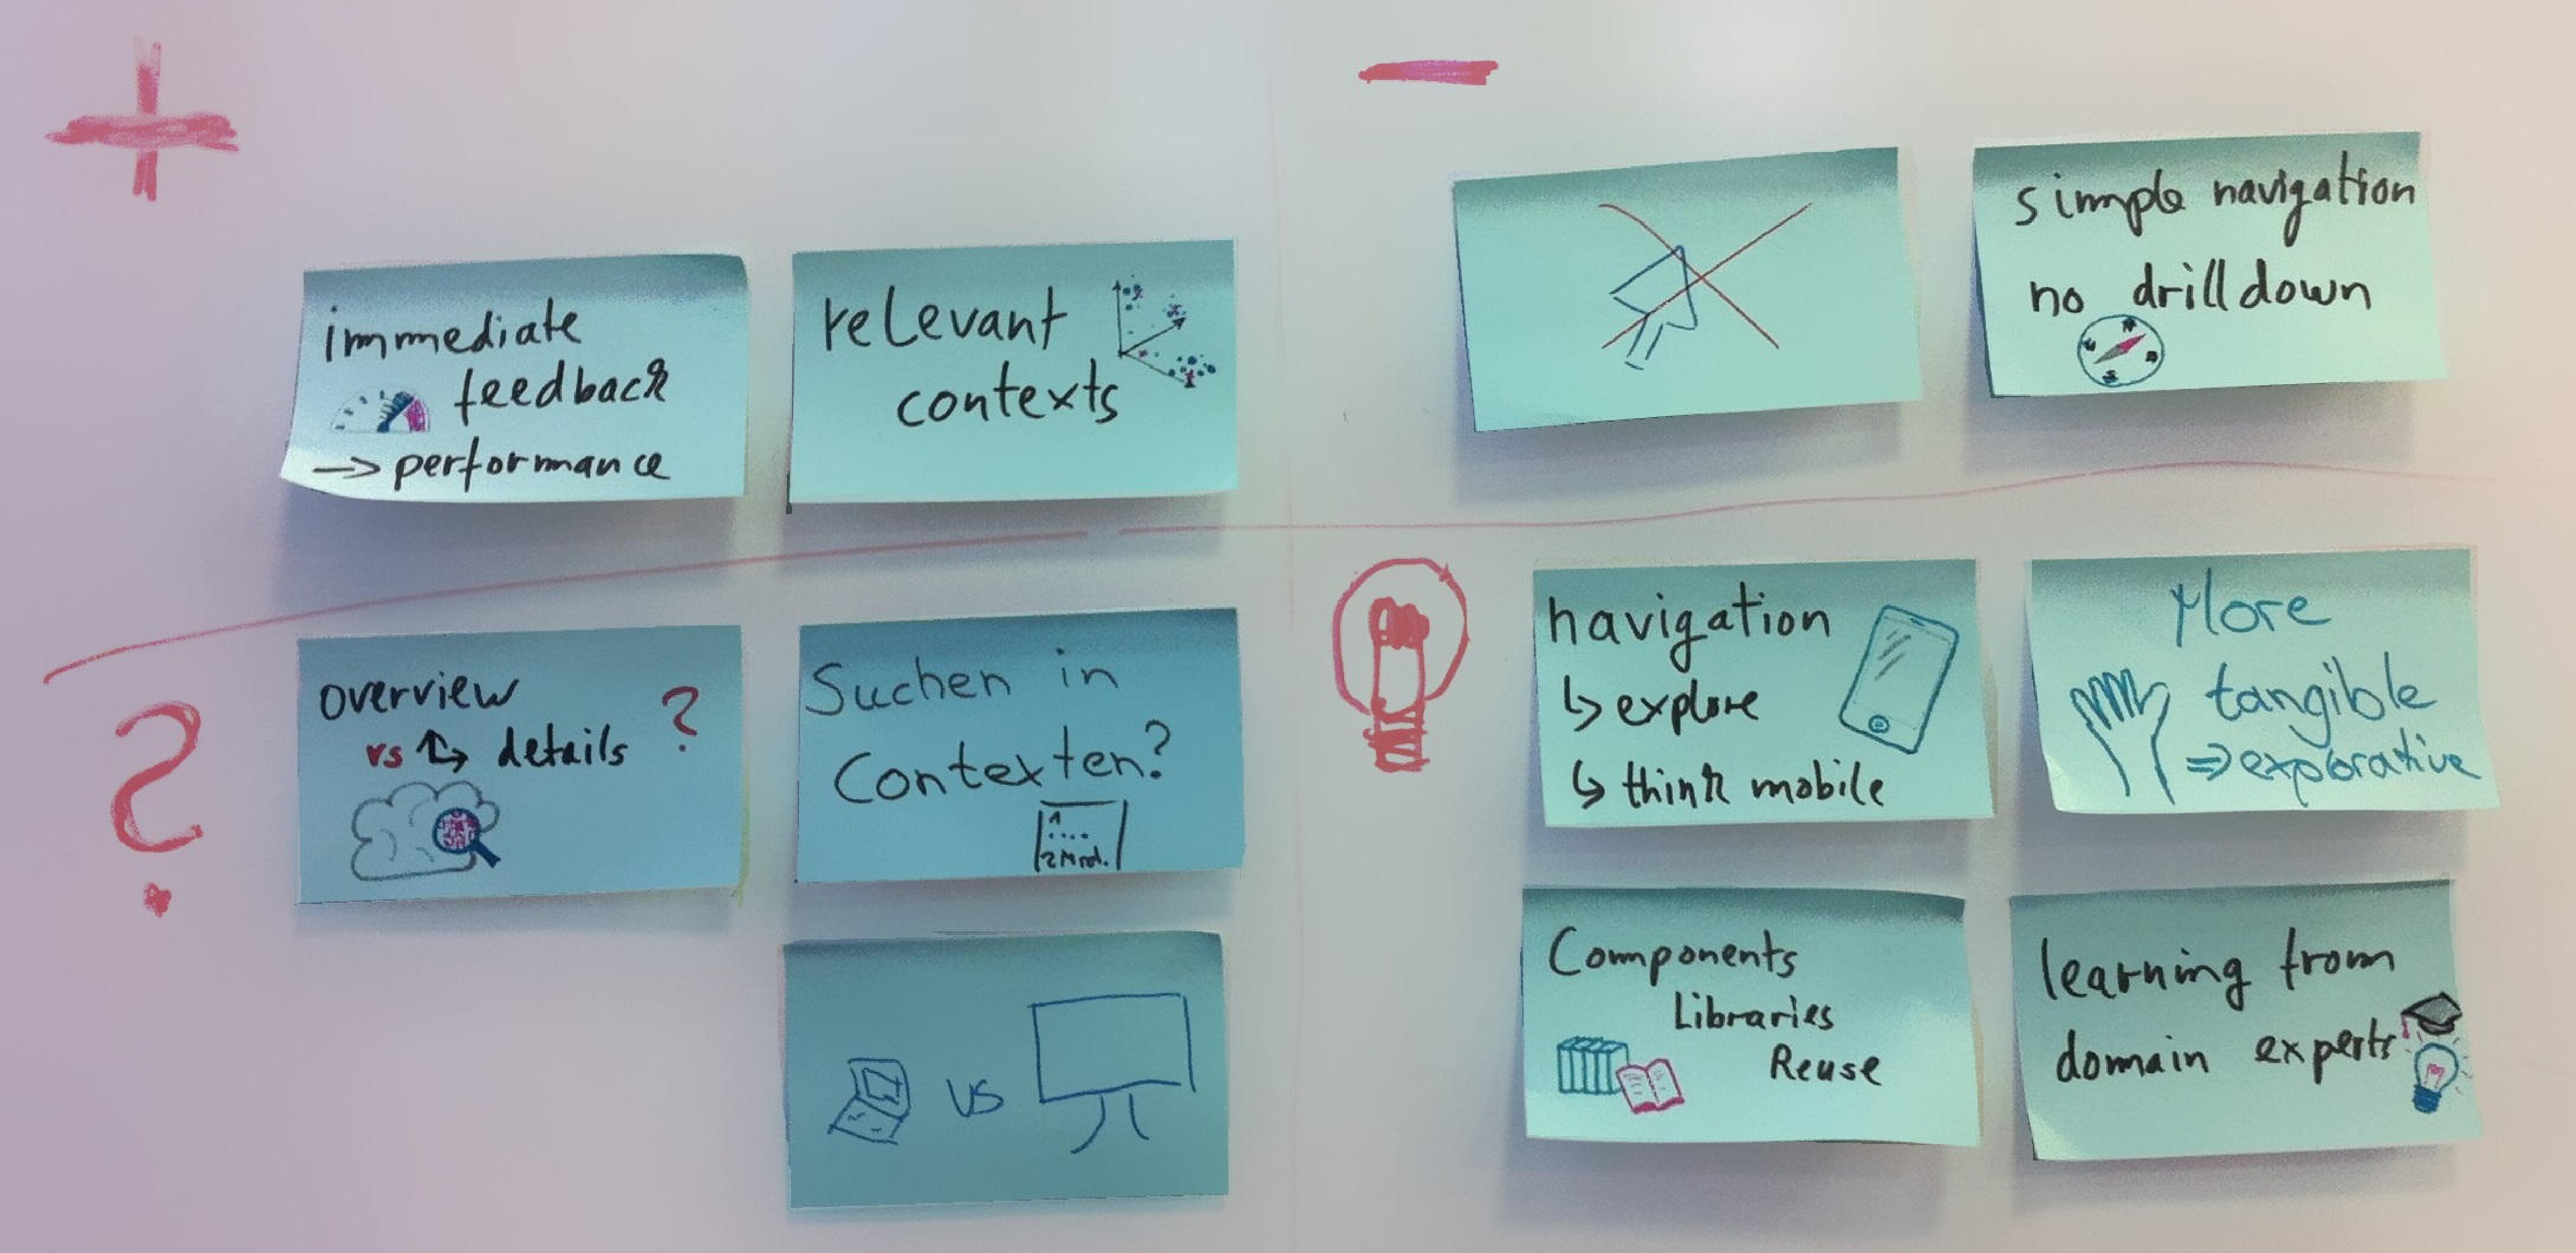
\includegraphics[width=1.0\linewidth]{images/user_feedback}
    \caption{User feedback captured on Post-Its and arranged in the feedback panel with positive and negative feedback as well as questions and new ideas.}
    % #selfrespect
    \label{fig:user_feedback}
\end{centering}
\end{figure}